\documentclass{article}
\usepackage[top=2.5cm, left=3cm, right=3cm, bottom=4.0cm]{geometry}
\usepackage{graphicx} 
\usepackage{amsfonts,amsmath,amssymb}
\usepackage{array}
\usepackage{tabularray}
\usepackage[utf8]{inputenc}
\usepackage[T1]{fontenc}
\usepackage{csquotes}
\usepackage{alphabeta}
\usepackage{url}
\usepackage{hyperref}
\usepackage{esint}

\renewcommand{\figurename}{Γράφημα}

\begin{document}
\begin{table}[ht]
    \begin{tblr}{
        @{}X[l, valign=b]X[c, valign=b]X[r, valign=b]@{}
    }

    \hline
    % First line, course info
    \SetCell[c=2]{l}{[ΘΠ04] Παράλληλα Συστήματα} & & {2024-25} \\ 
    \hline
    {} & {} & {} \\

    % Title
    \SetCell[c=3]{c}{ \Large \textbf{Εργασία 2 - Προγραμματισμός με OpenMP} } \\
    {} & {} & {} \\

    % Name Surname, Student ID
    \hline
    \SetCell[c=3]{c}{ \textbf{Ονοματεπώνυμο:} Μάριος Γιαννόπουλος } \\
    \SetCell[c=3]{c}{ \textbf{A.M.:} 1115200000032} \\
    \hline

    \end{tblr}
\end{table}
\section*{Γενικές Πληροφορίες}

\subsection*{Υπολογιστικό Σύστημα}
Όλο το έργο υλοποιήθηκε στο ίδιο υπολογιστικό περιβάλλον:
\begin{itemize}
    \item \textbf{Όνομα Υπολογιστικού Συστήματος:} Linux12
    \item \textbf{Επεξεργαστής:} Intel(R) Core(TM) i5-6500 CPU @ 3.20GHz
    \item \textbf{Αριθμός Πυρήνων:} 4
    \item \textbf{Λειτουργικό Σύστημα:} Linux Ubuntu 20.04.2 LTS
    \item \textbf{Έκδοση Μεταγλωττιστή:} gcc (Ubuntu 9.4.0-1ubuntu1~20.04.2) 9.4.0
\end{itemize}

\subsection*{Οδηγίες Εκτέλεσης Python Scripts}
Για την εκτέλεση των Python scripts που επεξεργάζονται τα αποτελέσματα, ακολουθήστε τα εξής βήματα:
\begin{enumerate}
    \item Μεταβείτε στον φάκελο \path{scripts}.
    \item Εγκαταστήστε τις απαραίτητες βιβλιοθήκες:
    \begin{verbatim}
    pip install -r requirements.txt
    \end{verbatim}
    \item Εκτελέστε το script που σας ενδιαφέρει:
    \begin{verbatim}
    python <test_script>.py
    \end{verbatim}
\end{enumerate}
\textbf{Σημείωση:} Όλα τα αποτελέσματα στα γραφήματα είναι από την εκτέλεση των πειραμάτων στο εργαστήριο Linux. Κάθε πείραμα εκτελέστηκε 5 φορές και τα αποτελέσματα αναφέρονται στο μέσο όρο των επαναλήψεων.
\section*{Άσκηση 2.1}
\subsection*{Εισαγωγή}
Σκοπός της παρούσας εργασίας είναι η παραλληλοποίηση του Παιχνιδιού της Ζωής (Game of Life) με χρήση της βιβλιοθήκης OpenMP. Το παιχνίδι, που σχεδιάστηκε από τον John Conway το 1970, είναι ένα μαθηματικό μοντέλο τοπικών κανόνων που παράγει πολύπλοκα μοτίβα. Στο πλαίσιο της εργασίας, υλοποιήθηκε τόσο σειριακή όσο και παράλληλη έκδοση του αλγορίθμου, ενώ τα πειράματα εκτελέστηκαν σε διαφορετικά μεγέθη πλεγμάτων και αριθμούς νημάτων.
\subsection*{Συγχρονισμός}
Για την υλοποίηση της παράλληλης έκδοσης χρησιμοποιήθηκαν οι οδηγίες του OpenMP για την κατανομή του έργου στα διαθέσιμα νήματα. Λόγω της ανεξαρτησίας των υπολογισμών για κάθε κελί (εκτός από την ανάγνωση των γειτονικών κυψελών), δεν απαιτείται πρόσθετος συγχρονισμός μεταξύ των νημάτων. Οι γενιές ενημερώνονται ταυτόχρονα χωρίς αλληλεξάρτηση, οπότε η παραλληλία εφαρμόζεται χωρίς την ανάγκη συγχρονισμού ή κλειδώματος των δεδομένων.
\subsection*{Πειραματική Διαδικασία}
\begin{itemize}
    \item \textbf{Παραμετροποίηση:}
    \begin{itemize}
        \item Μέγεθος πλέγματος: $64 \times 64$, $1024 \times 1024$, $4096 \times 4096$.
        \item Αριθμός γενιών: 1000.
        \item Αριθμός νημάτων: 2, 4, 8, 16.
    \end{itemize}
    \item \textbf{Εκτέλεση:}
    \begin{itemize}
        \item Τα πειράματα εκτελέστηκαν 5 φορές για κάθε συνδυασμό παραμέτρων.
        \item Καταγράφηκε ο χρόνος εκτέλεσης για κάθε πείραμα.
        \item Τα δεδομένα αποθηκεύτηκαν σε CSV αρχείο.
    \end{itemize}
    \item \textbf{Αυτοματοποίηση:}
    \begin{itemize}
        \item Αναπτύχθηκαν Python scripts για την εκτέλεση των πειραμάτων και την καταγραφή των δεδομένων.
        \item Χρησιμοποιήθηκαν Python scripts για την επεξεργασία των αποτελεσμάτων και τη δημιουργία γραφημάτων.
    \end{itemize}
\end{itemize}
\subsection*{Αποτελέσματα}
\begin{itemize}
    \item \textbf{Σύγκριση Σειριακού και Παράλληλου Αλγορίθμου:}
    \begin{itemize}
        \item Για το πλέγμα 64x64, η σειριακή εκτέλεση έχει χρόνο εκτέλεσης γύρω από 0.38s. Ωστόσο, η παράλληλη εκτέλεση με 2 νήματα αποδίδει καλύτερα με μέσο χρόνο περίπου 0.32s, ενώ για περισσότερα νήματα (4, 8, 16) παρατηρείται αύξηση του χρόνου εκτέλεσης λόγω του overhead της παραλληλοποίησης. Αυτό δείχνει ότι για μικρά πλέγματα η παραλληλοποίηση μπορεί να έχει μικρότερο όφελος.
        \item Για το πλέγμα 1024x1024, η σειριακή εκτέλεση έχει μέσο χρόνο περίπου 40.3s. Η παράλληλη εκτέλεση επιταχύνει τη διαδικασία, με 2 νήματα να χρειάζονται περίπου 20.8s και 16 νήματα περίπου 16s, υποδεικνύοντας σημαντική βελτίωση στους χρόνους εκτέλεσης με την αύξηση του αριθμού των νημάτων.
        \item Για το πλέγμα 4096x4096, η σειριακή εκτέλεση απαιτεί περίπου 643.3s. Με την παράλληλη εκτέλεση, οι χρόνοι μειώνονται σημαντικά: 331.2s με 2 νήματα και 234.6s με 16 νήματα, επιβεβαιώνοντας τη μεγάλη αποδοτικότητα της παραλληλοποίησης για μεγάλα πλέγματα.
    \end{itemize}
\end{itemize}
\subsection*{Γραφήματα}
Το παρακάτω γράφημα παρουσιάζει τη σχέση μεταξύ του μεγέθους του πλέγματος, του αριθμού των νημάτων και του χρόνου εκτέλεσης:
\begin{figure}[h]
    \centering
    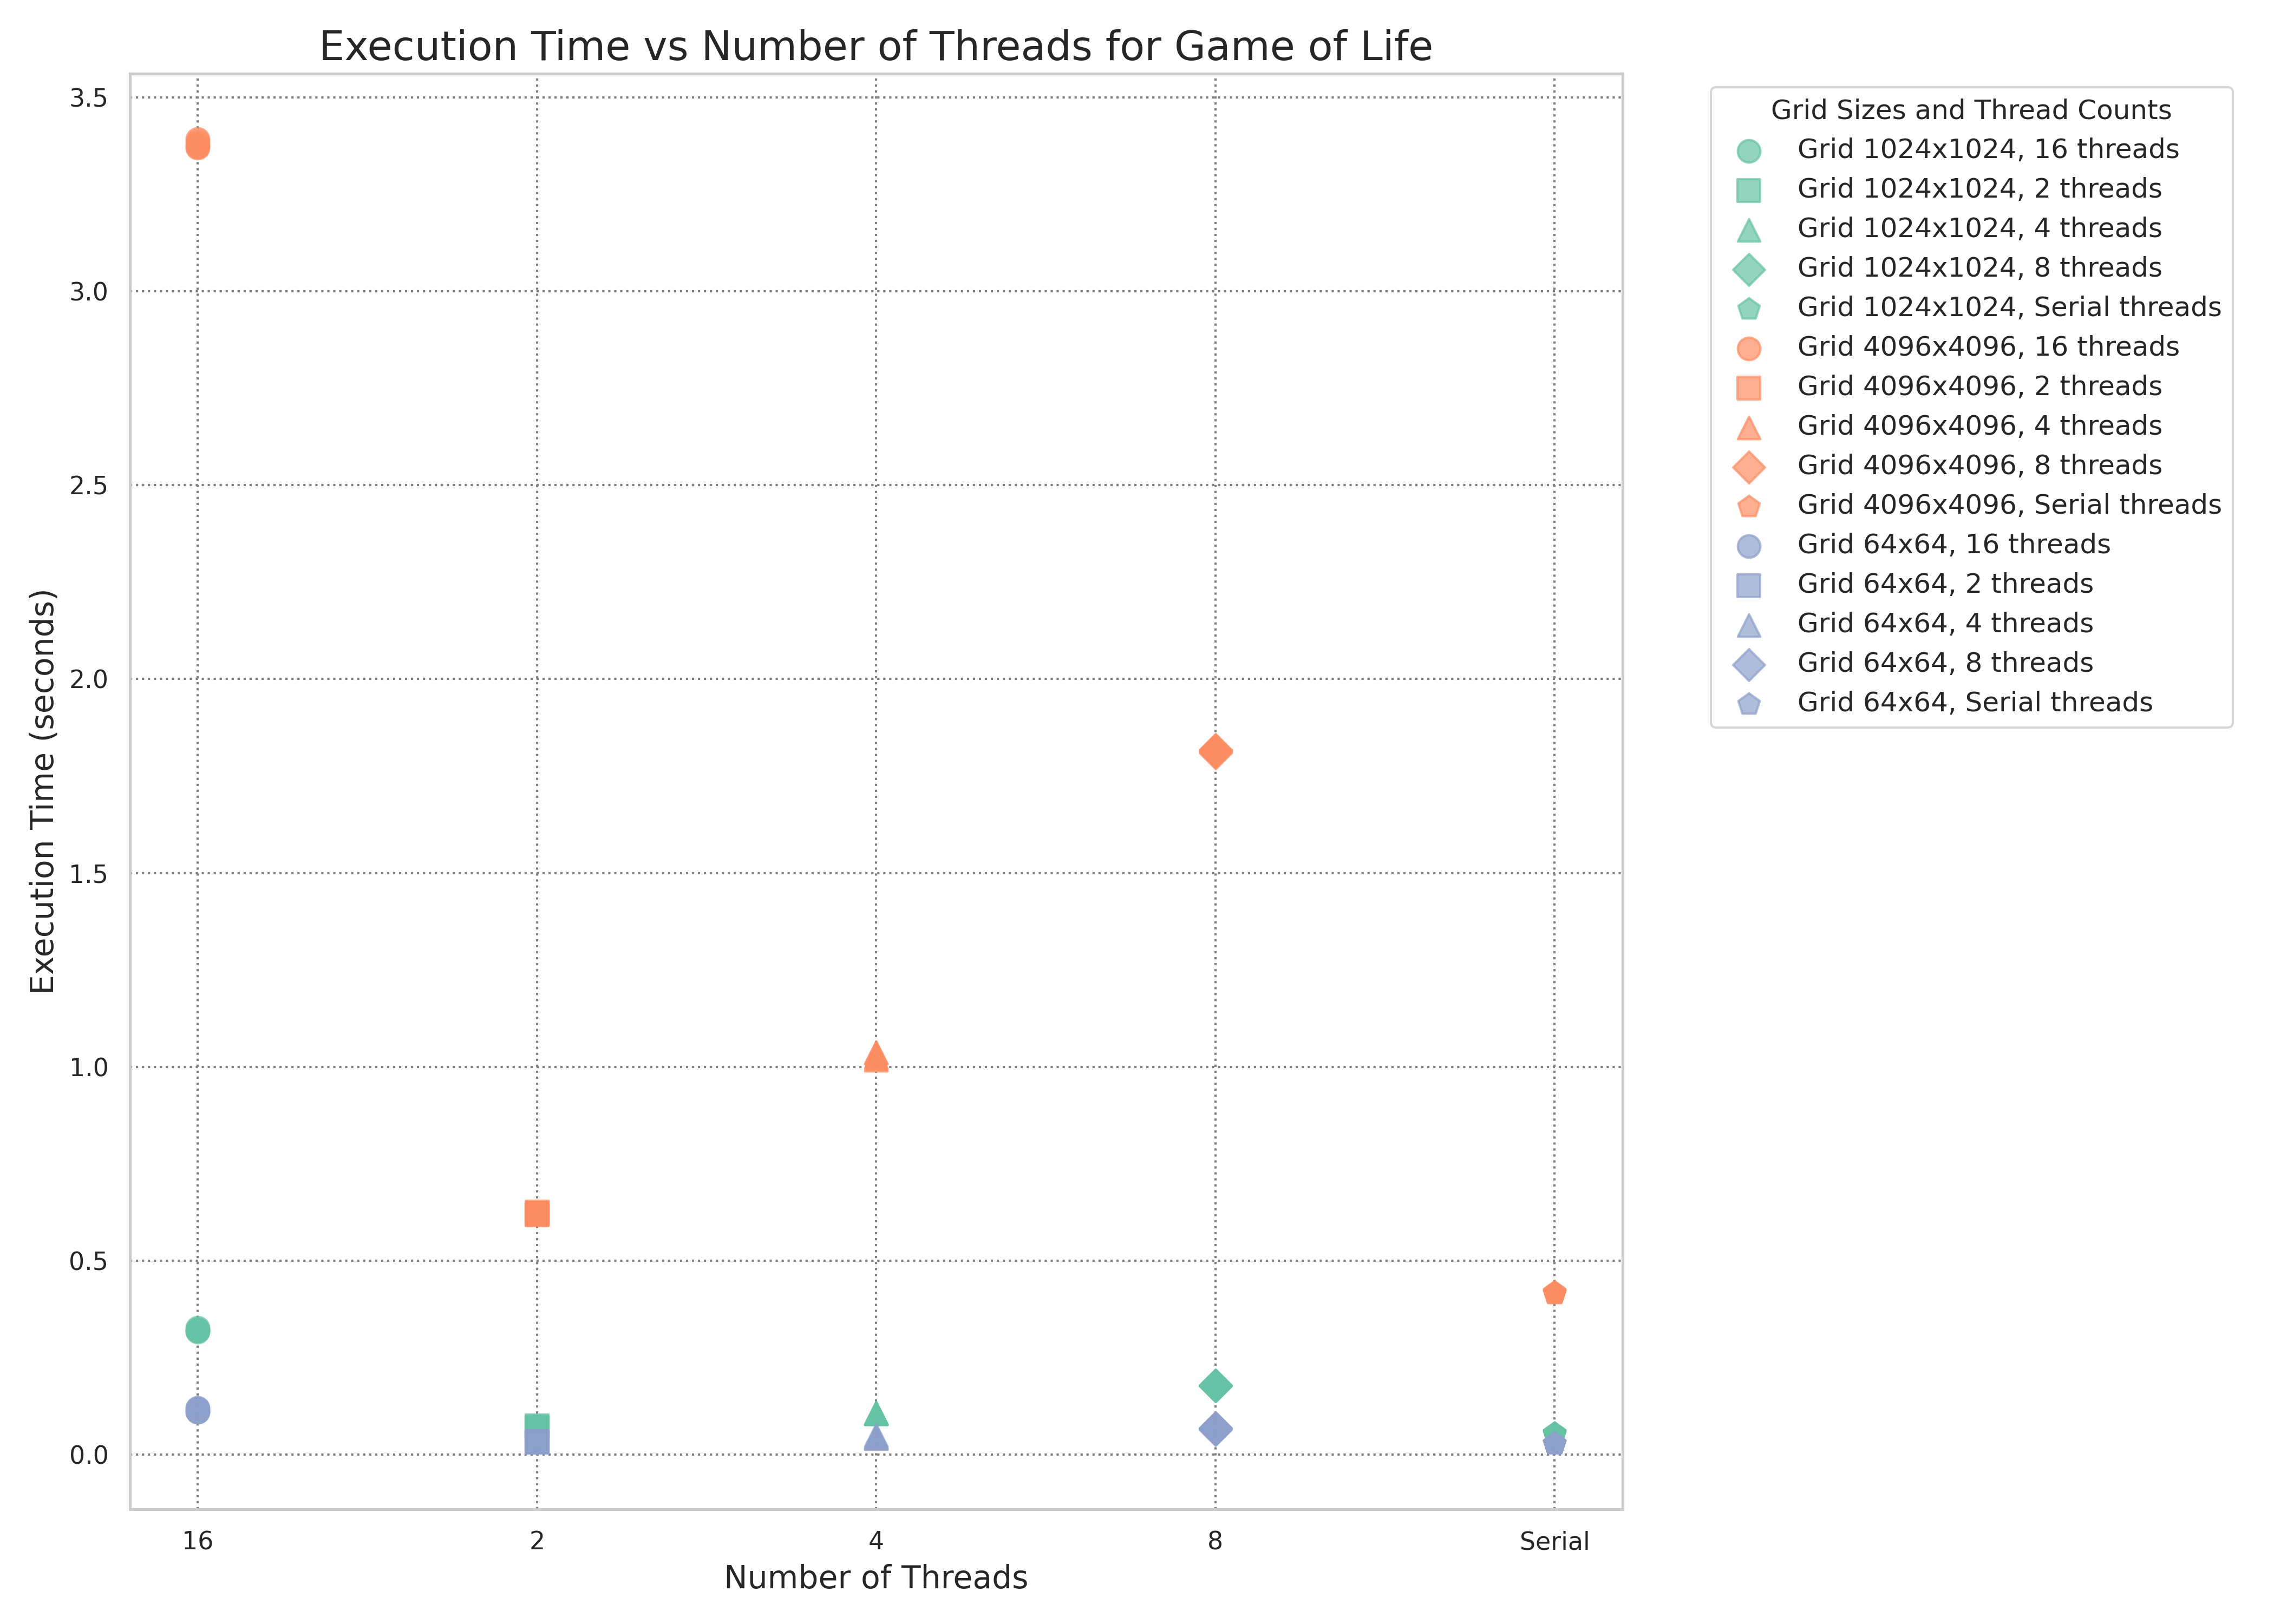
\includegraphics[width=1\textwidth]{game_of_life_results.png}
    \caption{Χρόνος Εκτέλεσης ανά Μέγεθος Πλέγματος και Αριθμό Νημάτων}
\end{figure}
\subsection*{Συμπεράσματα}
\begin{enumerate}
    \item Η παραλληλοποίηση είναι αποδοτική για μεγάλα μεγέθη πλεγμάτων, όπως φαίνεται από τη σημαντική μείωση του χρόνου εκτέλεσης στα πλέγματα 1024x1024 και 4096x4096, με την αύξηση του αριθμού των νημάτων.
    \item Για μικρά πλέγματα (όπως το 64x64), η παραλληλοποίηση με 2 νήματα προσφέρει κάποιες βελτιώσεις, αλλά για περισσότερα νήματα το overhead της παραλληλοποίησης επηρεάζει αρνητικά την απόδοση.
    \item Η απόδοση του αλγορίθμου περιορίζεται από τον αριθμό των διαθέσιμων πυρήνων του επεξεργαστή και το μέγεθος του πλέγματος, με την παραλληλοποίηση να αποδίδει καλύτερα σε μεγαλύτερους υπολογιστικούς πόρους και μεγαλύτερα δεδομένα.
    \item Για μικρά πλέγματα, η σειριακή έκδοση παραμένει αποδοτικότερη λόγω του overhead της παραλληλοποίησης.
\end{enumerate}
Η εργασία κατέδειξε τη σημασία της παραλληλοποίησης για μεγάλα προβλήματα, αλλά και τους περιορισμούς της λόγω του hardware.
\section*{Άσκηση 2.2}
\subsection*{Εισαγωγή} 
Η παρούσα εργασία εξετάζει την παραλληλοποίηση της διαδικασίας επίλυσης γραμμικών συστημάτων με τη χρήση της απαλοιφής Gauss και της αντικατάστασης προς τα πίσω. Η απαλοιφή Gauss μετατρέπει ένα σύστημα σε άνω τριγωνική μορφή, ενώ η αντικατάσταση προς τα πίσω υπολογίζει τις λύσεις. Η εργασία περιλαμβάνει σειριακές και παράλληλες υλοποιήσεις τόσο για τον \textit{"κατά γραμμή"} όσο και για τον \textit{"κατά στήλη"} αλγόριθμο. Η αξιολόγηση των υλοποιήσεων γίνεται μέσω πειραμάτων σε διάφορα μεγέθη συστημάτων και αριθμούς νημάτων.
\subsection*{Προσεγγίσεις Παραλληλοποίησης} 
\begin{enumerate} 
    \item \textbf{Αλγόριθμος "Κατά Γραμμή":} 
    \begin{itemize} 
        \item Ο εξωτερικός βρόχος που διατρέχει τις γραμμές μπορεί να παραλληλοποιηθεί. 
        \item Ο εσωτερικός βρόχος παρουσιάζει εξαρτήσεις δεδομένων που καθιστούν την παραλληλοποίησή του πιο περίπλοκη. 
    \end{itemize} 
    \item \textbf{Αλγόριθμος "Κατά Στήλη":} 
    \begin{itemize} 
        \item Ο εξωτερικός βρόχος δεν παρουσιάζει εξαρτήσεις δεδομένων και παραλληλοποιείται εύκολα. 
        \item Ο εσωτερικός βρόχος επηρεάζεται από την εξάρτηση μεταξύ των στηλών, γεγονός που απαιτεί προσεκτικό χειρισμό. 
    \end{itemize} 
\end{enumerate} 
Για την παραλληλοποίηση, χρησιμοποιήθηκε το OpenMP, αξιοποιώντας οδηγίες όπως \verb|#pragma omp parallel for| για τον έλεγχο των βρόχων.
\subsection*{Πειραματική Διαδικασία} 
\begin{itemize} 
    \item \textbf{Παραμετροποίηση:} 
    \begin{itemize} 
        \item Μέγεθος συστήματος ($n$): 100, 1000, 5000, 10000. 
        \item Αριθμός νημάτων: 2, 4, 8, 16. \item Τύποι Αλγορίθμων: 
        \begin{itemize} \item "Κατά Γραμμή" και "Κατά Στήλη". 
            \item Σειριακή και Παράλληλη Υλοποίηση. 
        \end{itemize} 
        \item Χρονοπρογραμματισμός (Schedule): static, dynamic, guided, runtime. 
    \end{itemize} 
    \item \textbf{Διαδικασία Εκτέλεσης:} 
    \begin{itemize} 
        \item Κάθε πείραμα εκτελέστηκε 5 φορές και μετρήθηκε ο μέσος χρόνος εκτέλεσης. 
        \item Τα δεδομένα αποθηκεύτηκαν σε CSV για ανάλυση. 
    \end{itemize} 
    \item \textbf{Αυτοματοποίηση:} 
    \begin{itemize} 
        \item Αναπτύχθηκαν scripts σε Python για την αυτοματοποίηση των πειραμάτων, την επεξεργασία των αποτελεσμάτων και τη δημιουργία γραφημάτων. 
    \end{itemize} 
\end{itemize}
\subsection*{Αποτελέσματα} 
\begin{itemize} 
    \item \textbf{Σύγκριση Σειριακού και Παράλληλου Αλγορίθμου:} 
    \begin{itemize} 
        \item Για μικρότερα μεγέθη συστημάτων, όπως $100x100$, η παράλληλη εκτέλεση δεν δείχνει σημαντική βελτίωση στον χρόνο εκτέλεσης λόγω του overhead της παραλληλοποίησης. Για παράδειγμα, με 2 νήματα στον "κατά γραμμή" αλγόριθμο και το static schedule, ο χρόνος εκτέλεσης για το $100x100$ πίνακα είναι 0.002366 (average).
        \item Για μεγαλύτερα μεγέθη πινάκων, όπως το $10000x10000$, παρατηρείται σημαντική βελτίωση με την παράλληλη εκτέλεση. Στο "κατά γραμμή" αλγόριθμο με guided schedule και 16 νήματα, ο χρόνος εκτέλεσης είναι 0.778388 (average).
    \end{itemize} 
    \item \textbf{Επιδόσεις ανά Schedule:} 
    \begin{itemize} 
        \item Το \textit{static} schedule παρουσιάζει σταθερή απόδοση για μικρότερα συστήματα, αλλά δεν προσφέρει τη βέλτιστη απόδοση για μεγαλύτερους πίνακες. Στο $10000x10000$ σύστημα, ο χρόνος εκτέλεσης με 16 νήματα και static schedule είναι 0.983888 (average).
        \item Το \textit{dynamic} schedule επιτρέπει ευελιξία για ανομοιόμορφα workloads, αλλά με μεγαλύτερο overhead. Στο ίδιο σύστημα, ο χρόνος με 16 νήματα και dynamic schedule είναι 0.892785 (average).
        \item Το \textit{guided} schedule παρέχει καλή ισορροπία, με καλύτερες επιδόσεις σε μεγάλους πίνακες. Στο $10000x10000$, ο χρόνος εκτέλεσης με guided schedule είναι 0.986361 (average).
        \item Το \textit{runtime} προσφέρει δυναμική ρύθμιση αλλά με κάποια αστάθεια, παρουσιάζοντας χρόνο 0.891547 (average) για το $10000x10000$ με 16 νήματα.
    \end{itemize} 
    \item \textbf{Γενικές Παρατηρήσεις:} 
    \begin{itemize} 
        \item Όσο αυξάνεται ο αριθμός των νημάτων, παρατηρείται μια σταθερή μείωση στον χρόνο εκτέλεσης για μεγάλους πίνακες. Ωστόσο, η βελτίωση είναι πιο εμφανής όταν τα μεγέθη των πινάκων είναι μεγαλύτερα (π.χ. $10000x10000$).
    \end{itemize} 
\end{itemize}
\subsection*{Γραφήματα} Τα παρακάτω γραφήματα παρουσιάζουν την επίδραση του μεγέθους του πίνακα, του αριθμού των νημάτων, του τύπου του αλγορίθμου και του schedule στον χρόνο εκτέλεσης:
\newpage
\begin{figure}[h] 
    \centering 
    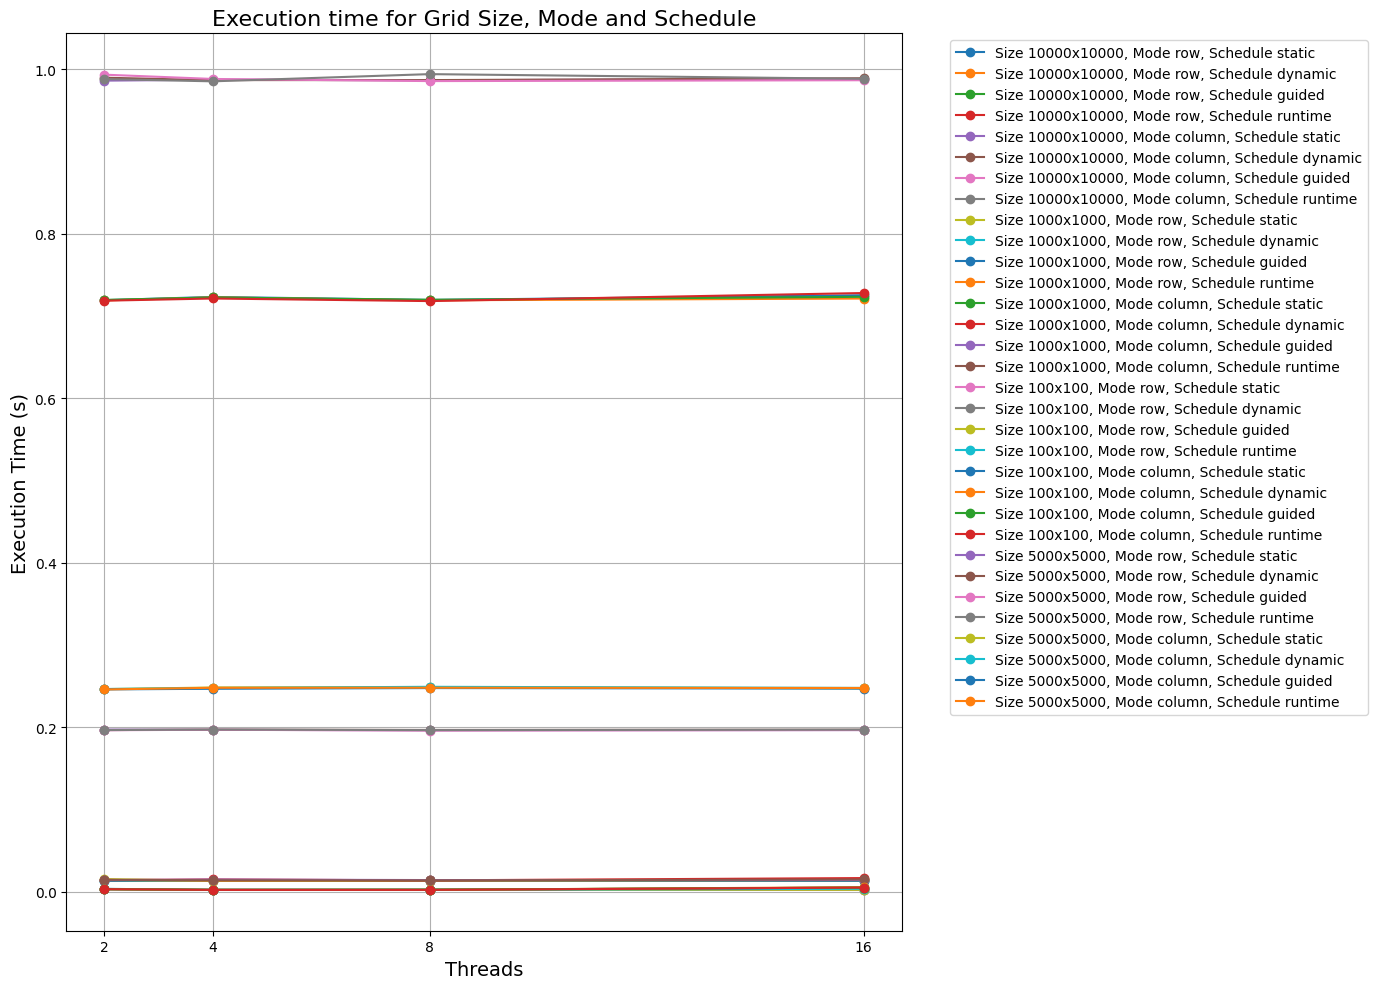
\includegraphics[width=0.8\textwidth]{gauss_elimination_results.png} 
    \caption{Χρόνος Εκτέλεσης κατά Μέγεθος Πίνακα, Αλγόριθμο και Τύπο Εκτέλεσης} 
\end{figure}
\newpage
\begin{figure}[h] 
    \centering 
    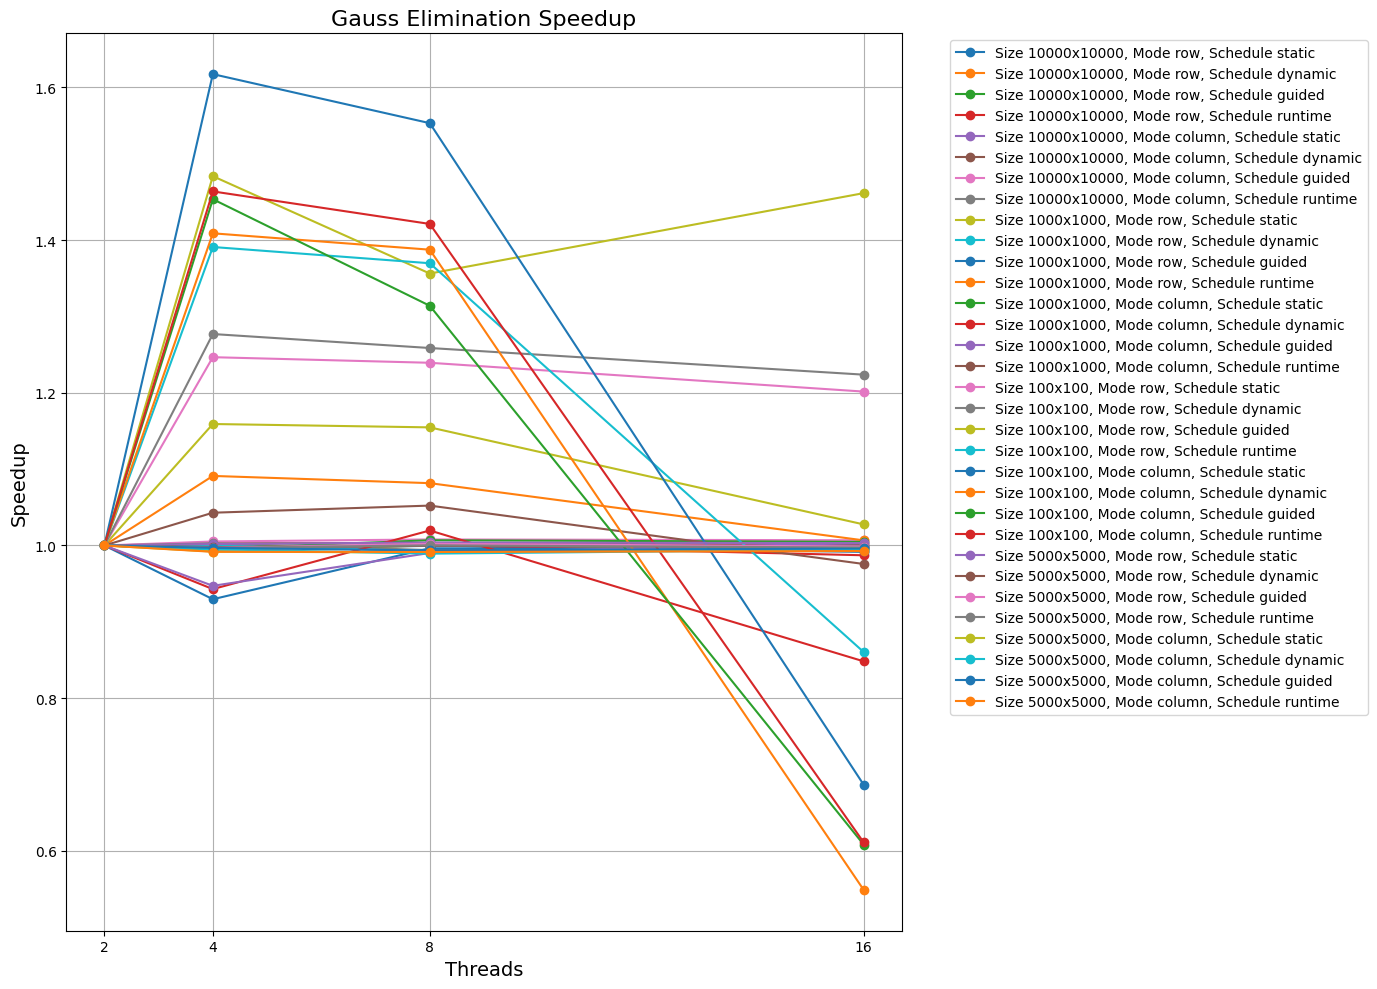
\includegraphics[width=0.8\textwidth]{gauss_elimination_speedup.png} 
    \caption{Επίδραση του Schedule στον Χρόνο Εκτέλεσης} 
\end{figure}
\subsection*{Συμπεράσματα} 
\begin{enumerate} 
    \item Η παραλληλοποίηση έχει σημαντική επίδραση στον χρόνο εκτέλεσης για μεγάλους πίνακες, όπως το $10000x10000$, όπου η χρήση 16 νημάτων μειώνει το χρόνο εκτέλεσης σημαντικά.
    \item Ο "κατά γραμμή" αλγόριθμος εμφανίζει καλύτερη απόδοση σε σχέση με τον "κατά στήλη", λόγω της μικρότερης πολυπλοκότητας και των λιγότερων εξαρτήσεων δεδομένων.
    \item Οι παράμετροι προγραμματισμού, όπως το schedule, έχουν σημαντική επίδραση στον χρόνο εκτέλεσης. Το guided και το static schedule προσφέρουν καλύτερη απόδοση σε μεγάλες διαστάσεις πινάκων, ενώ το dynamic και το runtime έχουν μεγαλύτερο overhead, ειδικά με μικρότερα συστήματα.
    \item Το μέγεθος του πίνακα και ο αριθμός των νημάτων επηρεάζουν σημαντικά την απόδοση. Για μεγαλύτερα συστήματα, η παραλληλοποίηση με υψηλό αριθμό νημάτων είναι ιδιαίτερα αποτελεσματική.
\end{enumerate} 
Η εργασία ανέδειξε την αποδοτικότητα της παραλληλοποίησης για μεγάλα συστήματα και τη σημασία της επιλογής του κατάλληλου schedule για τη βελτιστοποίηση του χρόνου εκτέλεσης.
\section*{Άσκηση 2.3} 
\subsection*{Εισαγωγή} Σκοπός της παρούσας εργασίας είναι η παραλληλοποίηση του Παιχνιδιού της Ζωής (Game of Life) χρησιμοποιώντας την οδηγία \texttt{task} της βιβλιοθήκης OpenMP. Η παραλληλοποίηση με τη χρήση της οδηγίας \texttt{task} επιτρέπει την κατανομή του υπολογιστικού έργου σε επιμέρους μονάδες εργασίας, οι οποίες μπορούν να εκτελούνται ασύγχρονα. Στο πλαίσιο της εργασίας, υλοποιήθηκε μια παράλληλη έκδοση του αλγορίθμου με την οδηγία \texttt{task}, η οποία συγκρίνεται με την προηγούμενη υλοποίηση της Άσκησης 2.1.
\subsection*{Συγχρονισμός} Για την υλοποίηση της παράλληλης έκδοσης με την οδηγία \texttt{task}, χρησιμοποιήθηκε η κατάλληλη κατανομή εργασιών μεταξύ των νημάτων, με στόχο την αποτελεσματική παράλληλη εκτέλεση. Κάθε γενιά του παιχνιδιού υποδιαιρείται σε μικρότερα καθήκοντα, τα οποία ανατίθενται σε διαφορετικά νήματα μέσω \texttt{task}. Η χρήση των \texttt{task} εξασφαλίζει τη σωστή εκτέλεση του αλγορίθμου χωρίς να απαιτείται άλλος συγχρονισμός μεταξύ των νημάτων.
\subsection*{Πειραματική Διαδικασία} 
\begin{itemize} 
    \item \textbf{Παραμετροποίηση:} 
    \begin{itemize} 
        \item Μέγεθος πλέγματος: $64 \times 64$, $1024 \times 1024$, $4096 \times 4096$. 
        \item Αριθμός γενιών: 1000. 
        \item Αριθμός νημάτων: 2, 4, 8, 16. 
    \end{itemize} 
    \item \textbf{Εκτέλεση:} 
    \begin{itemize} 
        \item Τα πειράματα εκτελέστηκαν 5 φορές για κάθε συνδυασμό παραμέτρων. 
        \item Καταγράφηκε ο χρόνος εκτέλεσης για κάθε πείραμα. 
        \item Τα δεδομένα αποθηκεύτηκαν σε CSV αρχείο. 
    \end{itemize} 
    \item \textbf{Αυτοματοποίηση:} 
    \begin{itemize} 
        \item Αναπτύχθηκαν Python scripts για την εκτέλεση των πειραμάτων και την καταγραφή των δεδομένων. 
        \item Χρησιμοποιήθηκαν Python scripts για την επεξεργασία των αποτελεσμάτων και τη δημιουργία γραφημάτων. 
    \end{itemize} 
\end{itemize}
\subsection*{Αποτελέσματα} 
\begin{itemize} 
    \item \textbf{Σύγκριση Σειριακού και Παράλληλου Αλγορίθμου (OpenMP task):} 
    \begin{itemize} 
        \item Για μικρά πλέγματα ($64 \times 64$), ο σειριακός αλγόριθμος ήταν ταχύτερος λόγω του overhead της παραλληλοποίησης. 
        \item Για μεγαλύτερα πλέγματα ($1024 \times 1024$ και $4096 \times 4096$), ο παράλληλος αλγόριθμος παρουσίασε σημαντική βελτίωση στον χρόνο εκτέλεσης. 
    \end{itemize} 
    \item \textbf{Επιτάχυνση:} 
    \begin{itemize} 
        \item Η απόδοση βελτιώθηκε με την αύξηση του αριθμού των νημάτων μέχρι να εξαντληθούν οι φυσικοί πόροι του επεξεργαστή. 
        \item Το μέγεθος του πλέγματος επηρέασε άμεσα την απόδοση, καθώς μεγαλύτερα πλέγματα επέτρεψαν την πλήρη αξιοποίηση της παραλληλίας. 
    \end{itemize} 
    \item \textbf{Γραμμικότητα της Κλιμάκωσης:}
    \begin{itemize}
        \item Παρατηρήθηκε γραμμική βελτίωση στην επιτάχυνση για μικρό αριθμό νημάτων. 
        \item Σε μεγαλύτερους αριθμούς νημάτων, η γραμμικότητα μειώθηκε λόγω αυξημένου synchronization overhead.
    \end{itemize}
\end{itemize}
\subsection*{Γραφήματα} 
Το παρακάτω γράφημα παρουσιάζει τη σχέση μεταξύ του μεγέθους του πλέγματος, του αριθμού των νημάτων και του χρόνου εκτέλεσης για την παράλληλη υλοποίηση με την οδηγία \texttt{task}: 
\begin{figure}[h] 
    \centering 
    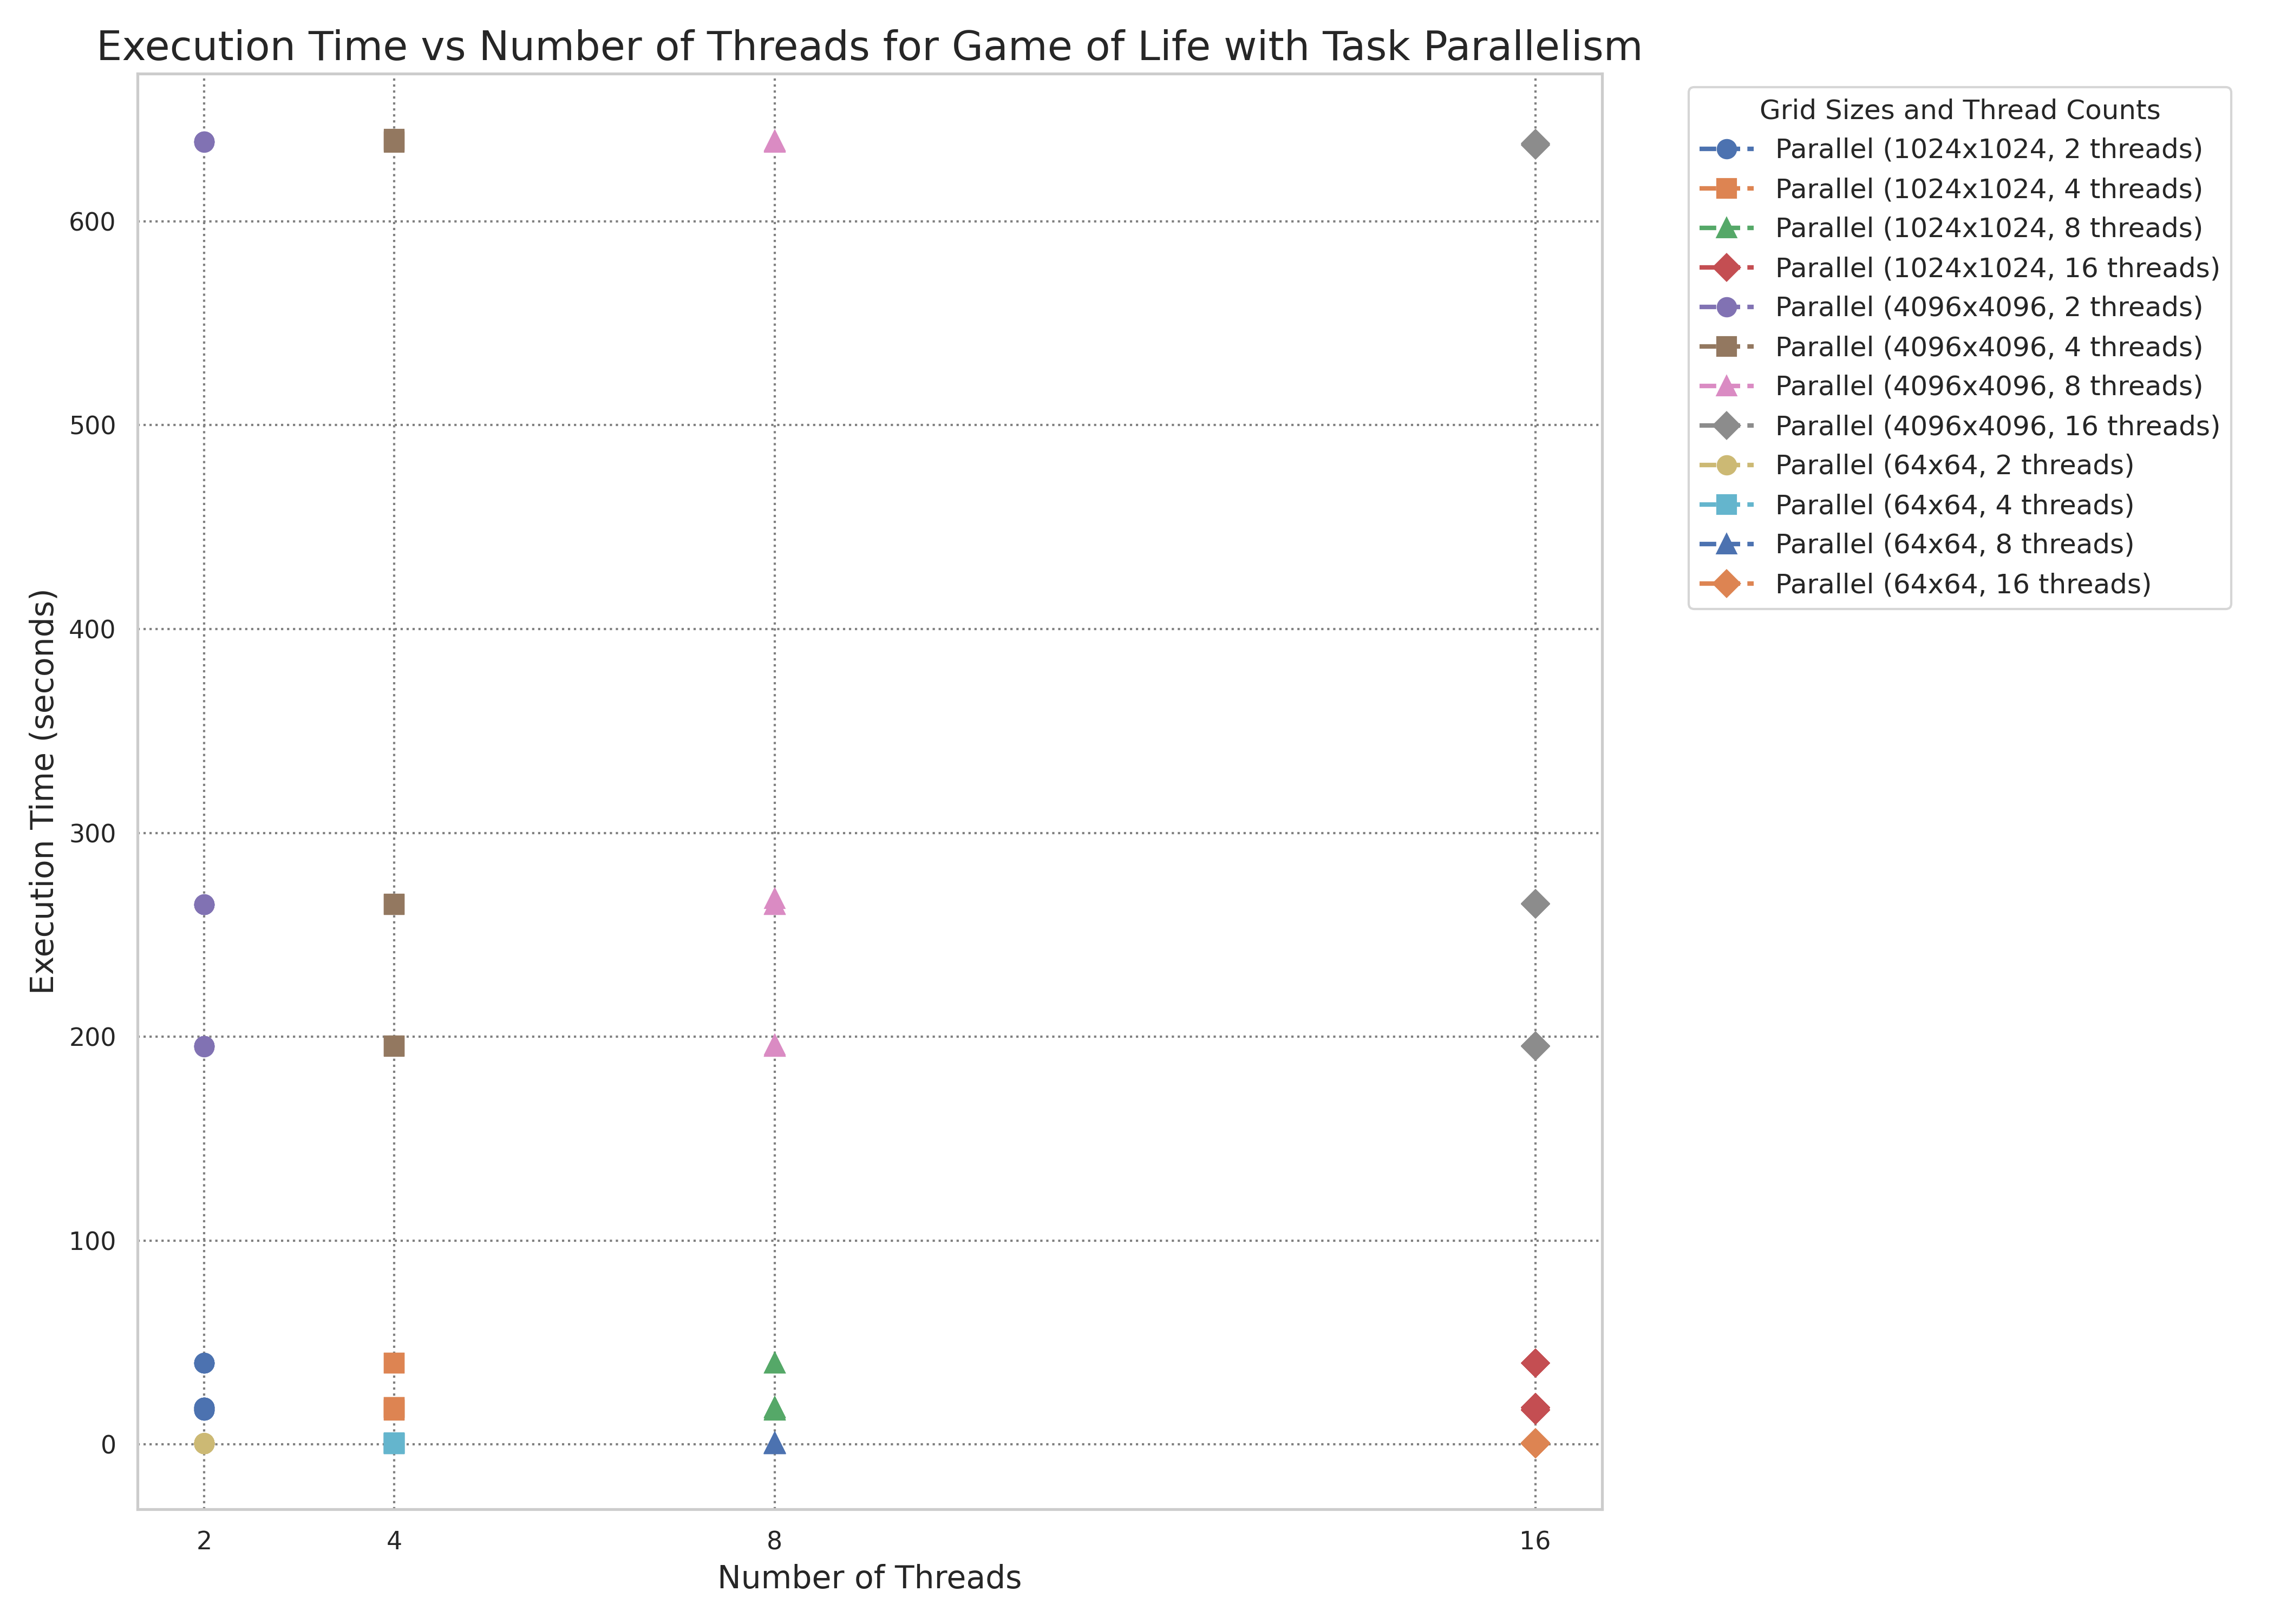
\includegraphics[width=1\textwidth]{game_of_life_tasks_results.png} 
    \caption{Χρόνος Εκτέλεσης ανά Μέγεθος Πλέγματος και Αριθμό Νημάτων με OpenMP Task} 
\end{figure}
\subsection*{Συμπεράσματα} 
\begin{enumerate} 
    \item Η χρήση της οδηγίας \texttt{task} στην παραλληλοποίηση του Game of Life προσφέρει σημαντικά πλεονεκτήματα για μεγάλα μεγέθη πλεγμάτων. 
    \item Η απόδοση της παραλληλοποίησης περιορίζεται από το hardware του συστήματος, συγκεκριμένα από τον αριθμό των διαθέσιμων πυρήνων και το synchronization overhead. 
    \item Για μικρά μεγέθη πλεγμάτων, η σειριακή έκδοση παραμένει πιο αποδοτική λόγω του υψηλού κόστους διαχείρισης των tasks. 
    \item Ο παράλληλος αλγόριθμος με \texttt{task} προσφέρει ευελιξία στη διαχείριση του υπολογιστικού έργου, αλλά απαιτεί προσεκτική ρύθμιση των παραμέτρων για τη μεγιστοποίηση της απόδοσης. 
\end{enumerate}
Η ανάλυση των αποτελεσμάτων κατέδειξε ότι η επιλογή παραλληλοποίησης πρέπει να γίνεται με βάση το μέγεθος του προβλήματος και τις δυνατότητες του συστήματος, επιβεβαιώνοντας την ευελιξία και την αποδοτικότητα της οδηγίας \texttt{task}.
\end{document}